\section{\'Arbres d'attaque et de défense}
	% Etoffer
	% Utiliser references

	% Theorie: un petit peu fort
    \subsection{Concept des arbres d'attaque et de défense}
        Le concept des arbres d'attaque a été introduit en 1999 par Bruce Schneier, un expert américain en sécurité informatique qui est parti du constat que des systèmes réputés "inviolables" se font briser en permanence \cite{doc_Schneier}. De plus, ces systèmes sont brisés non pas en passant au travers des défenses mises en place, mais par des méthodes d'accès qui n'avaient pas été imaginées par ses concepteurs, car ils n'avaient pas les outils pour dresser une liste exhaustive des manières d'attaquer leur système. Il a donc imaginé le concept des arbres d'attaque dans ce but : pouvoir réaliser un inventaire exhaustif des méthodes d'attaque sur un système, quel qu'il soit, afin de pouvoir en concevoir la défense de la manière la plus complète possible. Schneier a lui-même imaginé son modèle d'arbre d'attaque à partir du concept des "Arbres de défaillances", une méthodologie datant du début des années soixante dont le but est de pouvoir évaluer l'impact de la défaillance d'un composant sur le système dont il fait parti \cite{defaillanceTree}. 

        % Utiliser fig:arbre_exemple_1 pour expliquer le formalisme: plus visuel, plus clair
		Lors de ces recherches, Schneier a retenu un formalisme précis : une représentation des menaces sous la forme d'arbres. Ces arbres sont réalisés en se posant la question suivante : si l'attaquant veux atteindre tel objectif, qu'est ce que cela pré-suppose qu'il accomplisse d'abord ? Pour cela, on représente l'objectif principal à la racine de l'arbre (en haut), et l'on ajoute en descendant dans l'arbre des nœuds représentant des objectifs intermédiaires à réaliser et qui nous garantissent l'accomplissement de l'objectif principal. L'ajout de ces nœuds peut se faire sous deux formes distinctes : par disjonction ou conjonction. La disjonction correspond à des cas où la validation d'un seul des nœuds enfants valide le nœud parent (opération logique OU, représentée par des traits simples). La conjonction quant-à elle correspond à des cas où il faut valider l'ensemble des nœuds enfants pour valider le nœud parent (opération logique ET, représentée par des traits simples reliés entre eux par un arc). L'on fait ensuite découler de ces objectifs intermédiaires d'autres objectifs les validant et ainsi de suite, jusqu'à avoir les actions de base aux feuilles de l'arbre (en bas). Ensuite, il suffit de descendre dans l'arbre à partir d'un nœud pour savoir quelles sont les combinaisons d'actions possibles à effectuer pour atteindre le nœud. Les éléments (nœuds et feuilles) sont traditionnellement représentés par des ronds.

        L'arbre de la Figure \ref{fig:arbre_exemple_1} illustre ce formalisme : Objectif final à la racine, actions aux feuilles, et nœuds conjonctifs (besoin de la carte ET du code) et disjonctifs (par borne OU par internet).

        Enfin, le modèle des arbres d'attaques intègre la possibilité d'associer aux feuilles des valeurs représentatives de diverses informations sur l'accomplissement de l'action : coût, difficulté, probabilité, temps d'exécution, etc. Ces valeurs permettent alors de quantifier le "poids" du nœud dans l'arbre vis-à-vis de l'attaquant.  Il est alors possible à partir de ces valeurs de pouvoir quantifier ces mêmes informations pour les nœuds parents qui en découlent (par exemple en s'intéressant au coût financier pour l'attaquant, le coût de l'action d'un nœud OU peut prendre la valeur du coût minimal parmi ses nœuds enfants, tandis que dans le cas d'un nœud ET son coût sera leur somme), ce qui peut servir à l'attaquant pour choisir une stratégie d'attaque plutôt qu'une autre au vu de ses ressources.

        % A retravailler, pour l'integrer dans la description du formalisme.
		\begin{figure}
			\begin{center}
				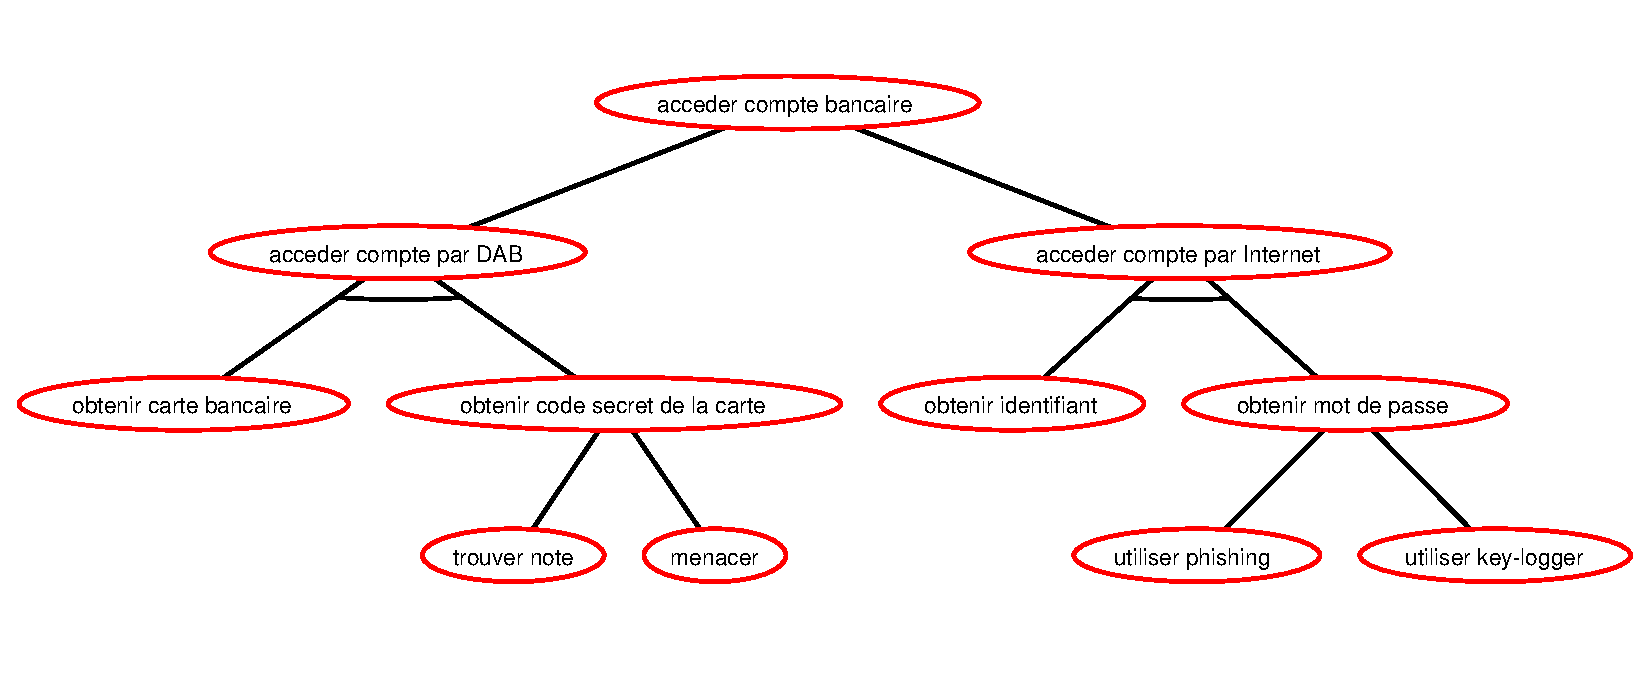
\includegraphics[width=0.8\textwidth]{figure/exemple1_rapport.pdf}
			\end{center}
			\caption{Arbre d'attaque}
			\label{fig:arbre_exemple_1}
		\end{figure}

		Depuis 1999, le concept des arbres d'attaque et de défense a évolué grâce à la contribution de personnes ayant étendu et amélioré le modèle de Schneier \cite{ADTreeKordy}. Ces personnes ont en particulier étendu le concept d'arbre d'attaque à celui d’arbre d’attaque et de défense (attack–defense tree ADTree), où sont également représentés les défenses mises en place et que le potentiel attaquant aura besoin de désactiver pour atteindre son but \cite{ADTreeOxford}. Les défenses sont traditionnellement représentés par des rectangles. Le même cas que précédemment pour lequel des défense auraient été mises en place pourrait correspondre à la figure \ref{fig:arbre_exemple_2} : Pour accéder au compte l'attaquant à besoin de désactiver l'authentificateur, même en possession du login ET du mot de passe.

        \begin{figure}
            \begin{center}
                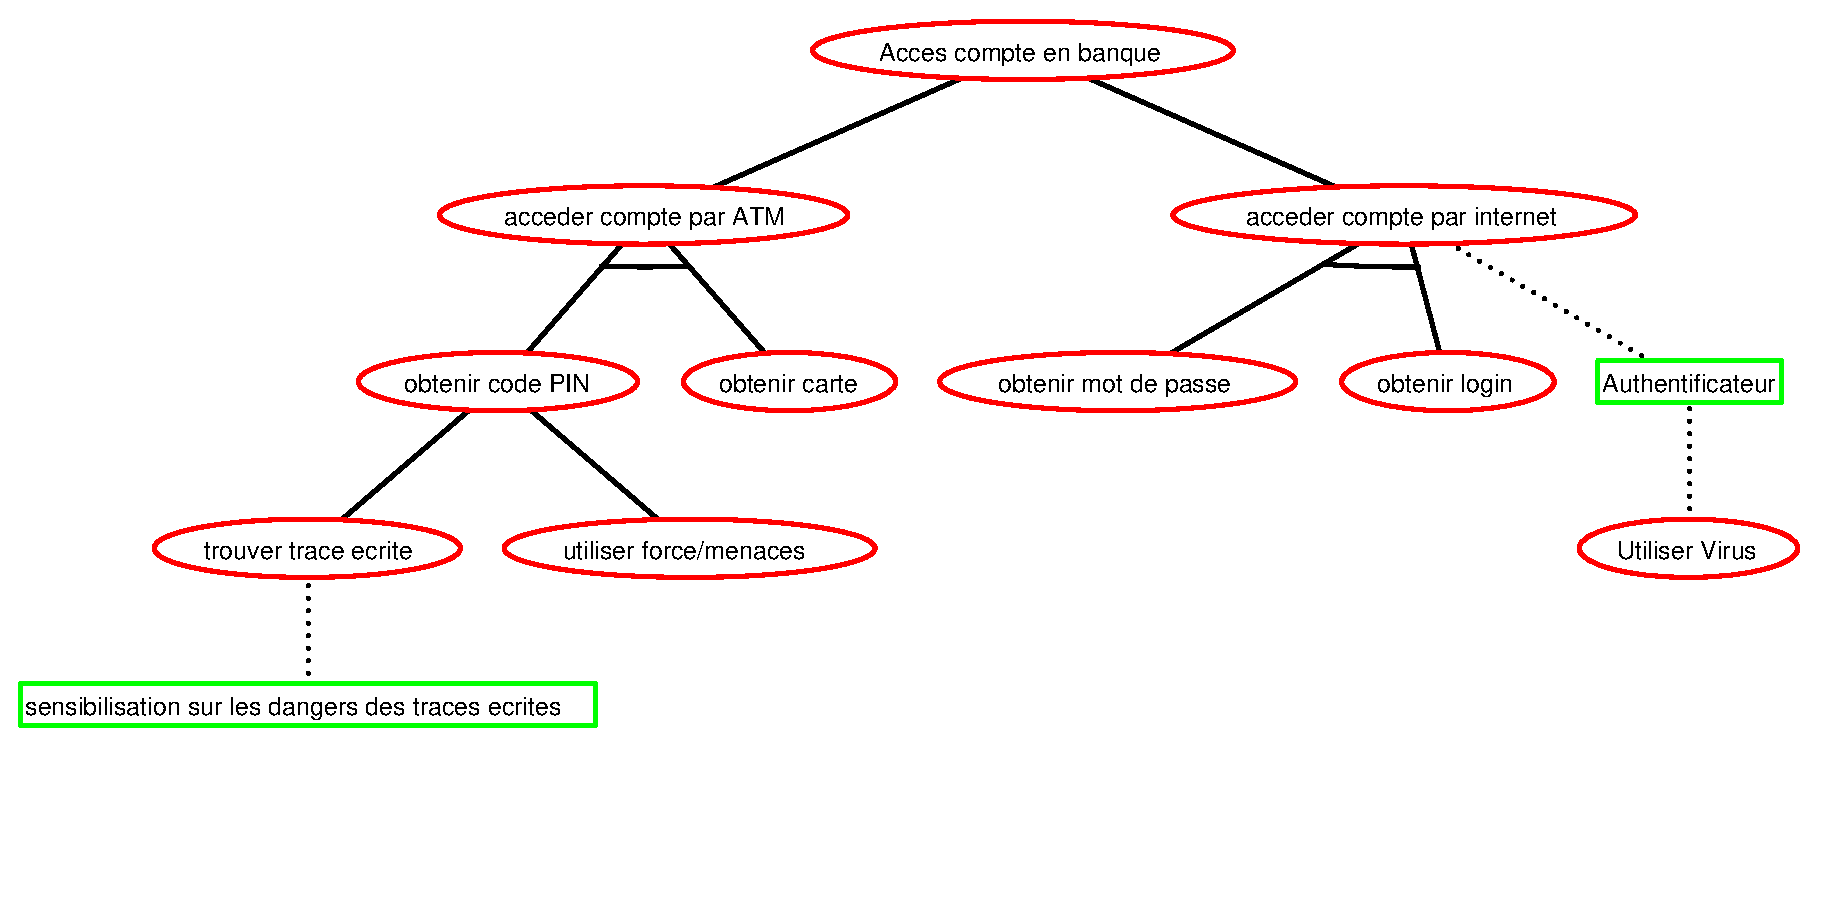
\includegraphics[width=1\textwidth]{figure/exemple2_rapport.pdf}
            \end{center}
            \caption{ADTree}
            \label{fig:arbre_exemple_2}
        \end{figure}

	\subsection{Implémentations des ADTree}
		Plusieurs logiciels implémentant le concept des arbres d'attaques ou des ADTree ont été développés. En voici quelques-uns :
        
        Logiciels propriétaires :
        \begin{itemize}
        \item SecurlTree : Logiciel de création et d'analyse d'arbres d'attaques développé par la société Amenaza \cite{SecurlTree}.
        \item ATTACKTREE+ : Logiciel de création et d'analyse d'arbres d'attaques développé par la société Isograph \cite{ATTACKTREE+}.
        \end{itemize}
        
        Logiciel Open-Source :
        \begin{itemize}
        \item ADTool: Logiciel développé par une équipe de chercheur de l'université du Luxembourg pour la modélisation d'ADTrees. Il s'agit d'un des logiciels que nous allons utiliser (plus de détails dans la Section \ref{sec:outils}) \cite{ADTool}.
        \end{itemize}

        \subsubsection{Synthèse}
            Aujourd'hui, les arbres d'attaques tels qu'introduits par Schneier sont utilisés par de nombreuses entreprises. Ceci est dû à l'avantage de pouvoir partir du point de vue de l'attaquant et donc de concentrer les efforts de défenses là où ils seront le plus utiles, à l'inverses d'un certain nombre d'autres stratégies de défense qui vont se concentrer seulement sur la défense du point de vue du défenseur (par exemple les arbres de défaillance), aboutissant forcément à une estimation des dangers incomplète et moins pertinente. 
            % Holy shit, faut reformuler ca

            Cela dit, un grand nombre de ces entreprises développent en interne leur propre logiciel de construction et d'analyse des ADTree sans toutefois utiliser ceux présents sur le marché. En effet, les solutions logicielles ne bénéficient pas d'une grande visibilité, peuvent être chères et ne sont pas forcément faciles à mettre en place. De plus, le nombre de logiciels implémentant les ADTree est assez réduit en comparaison de ceux implémentant les arbres d'attaques puisque nous avons pu en identifier un seul : ADTool. 

            Ceci étant, le développement peut être laborieux même en utilisant un logiciel dédié comme ADTool pour plusieurs raisons : le logiciel n’intègre pas d'arbres génériques ce qui rallonge le développement et oblige de modéliser plusieurs fois la même partie d'arbre, ne permet pas non plus de gérer la quantification de manière dynamique selon qui est l'attaquant, etc.

            Un grand nombre d'améliorations est donc possible : ce qui nous amène au cahier des charges.